%% Copernicus Publications Manuscript Preparation Template for LaTeX Submissions
%% ---------------------------------
%% This template should be used for copernicus.cls
%% The class file and some style files are bundled in the Copernicus Latex Package, which can be downloaded from the different journal webpages.
%% For further assistance please contact Copernicus Publications at: production@copernicus.org
%% https://publications.copernicus.org/for_authors/manuscript_preparation.html


%% Please use the following documentclass and journal abbreviations for preprints and final revised papers.

%% 2-column papers and preprints
\documentclass[tc, manuscript]{copernicus}
\usepackage{amsmath}


%% Journal abbreviations (please use the same for preprints and final revised papers)


% Advances in Geosciences (adgeo)
% Advances in Radio Science (ars)
% Advances in Science and Research (asr)
% Advances in Statistical Climatology, Meteorology and Oceanography (ascmo)
% Annales Geophysicae (angeo)
% Archives Animal Breeding (aab)
% ASTRA Proceedings (ap)
% Atmospheric Chemistry and Physics (acp)
% Atmospheric Measurement Techniques (amt)
% Biogeosciences (bg)
% Climate of the Past (cp)
% DEUQUA Special Publications (deuquasp)
% Drinking Water Engineering and Science (dwes)
% Earth Surface Dynamics (esurf)
% Earth System Dynamics (esd)
% Earth System Science Data (essd)
% E&G Quaternary Science Journal (egqsj)
% European Journal of Mineralogy (ejm)
% Fossil Record (fr)
% Geochronology (gchron)
% Geographica Helvetica (gh)
% Geoscience Communication (gc)
% Geoscientific Instrumentation, Methods and Data Systems (gi)
% Geoscientific Model Development (gmd)
% History of Geo- and Space Sciences (hgss)
% Hydrology and Earth System Sciences (hess)
% Journal of Bone and Joint Infection (jbji)
% Journal of Micropalaeontology (jm)
% Journal of Sensors and Sensor Systems (jsss)
% Magnetic Resonance (mr)
% Mechanical Sciences (ms)
% Natural Hazards and Earth System Sciences (nhess)
% Nonlinear Processes in Geophysics (npg)
% Ocean Science (os)
% Polarforschung - Journal of the German Society for Polar Research (polf)
% Primate Biology (pb)
% Proceedings of the International Association of Hydrological Sciences (piahs)
% Scientific Drilling (sd)
% SOIL (soil)
% Solid Earth (se)
% The Cryosphere (tc)
% Weather and Climate Dynamics (wcd)
% Web Ecology (we)
% Wind Energy Science (wes)


%% \usepackage commands included in the copernicus.cls:
%\usepackage[german, english]{babel}
%\usepackage{tabularx}
%\usepackage{cancel}
%\usepackage{multirow}
%\usepackage{supertabular}
%\usepackage{algorithmic}
%\usepackage{algorithm}
%\usepackage{amsthm}
%\usepackage{float}
%\usepackage{subfig}
%\usepackage{rotating}


\begin{document}

\title{Solid earth modulation of marine outlet glacier response}


% \Author[affil]{given_name}{surname}

\Author[1]{Andrew}{Hoffman}

%\Author[1]{Jessica}{Badgeley}
%\Author[2]{Katie}{Brennen}
%\Author[3]{John}{Christian}
%\Author[4]{Natalya}{Gomez}
%\Author[1]{Gerard}{Roe}

\affil[1]{Department of Earth and Space Sciences, University of Washington, Seattle, Washington, USA}

%\affil[2]{Department of Atmospheric Sciences, University of Washington, Seattle, Washington, USA}

%\affil[3]{School of Earth and Atmospheric Sciences, Georgia Institute of Technology, Atlanta, Georgia, USA }

%\affil[4]{Department of Earth and Planetary Sciences, McGill University, Montreal, Quebec, Canada }


%% The [] brackets identify the author with the corresponding affiliation. 1, 2, 3, etc. should be inserted.

%% If an author is deceased, please mark the respective author name(s) with a dagger, e.g. "\Author[2,$\dag$]{Anton}{Smith}", and add a further "\affil[$\dag$]{deceased, 1 July 2019}".

%% If authors contributed equally, please mark the respective author names with an asterisk, e.g. "\Author[2,*]{Anton}{Smith}" and "\Author[3,*]{Bradley}{Miller}" and add a further affiliation: "\affil[*]{These authors contributed equally to this work.}".


\correspondence{hoffmaao@uw.edu}

\runningtitle{Solid earth modulation of marine outlet glacier response and Heinrich events}

\runningauthor{Hoffman et al.}





\received{}
\pubdiscuss{} %% only important for two-stage journals
\revised{}
\accepted{}
\published{}

%% These dates will be inserted by Copernicus Publications during the typesetting process.


\firstpage{1}

\maketitle



\begin{abstract}
The dynamics of marine-terminating outlet glaciers and the solid earth are of fundamental interest in glaciology.
In this study, we analyze the response of a coupled marine outlet glacier-bedrock system to different sources of climate forcing.
We find that isostacy fundamentally changes the response of marine outlet glacier systems to surface-mass-balance forcing applied over the interior and the oceanic forcing applied at the grounding line.
The reduced model is shown to emulate the behavior of more complex numerical models of ice flow.
Together, these models demonstrate that ocean forcing first engages the fast, local response, and then the slow adjustment of interior ice, whereas surface-mass-balance forcing is dominated by the slow interior adjustment.
We also demonstrate the importance of the timescales of stochastic forcing for assessing the natural variability of outlet glaciers, highlighting that decadal persistence in ocean variability can affect the behavior of outlet glaciers on centennial and longer timescales.
Finally, we show that these transient responses have important implications for: attributing observed glacier changes to natural or anthropogenic influences; the future change already committed by past forcing; and the impact of past climate changes on the preindustrial glacier state, against which current and future anthropogenic influences are assessed.
\end{abstract}


\section{Introduction} 
Ice-sheet mass change in Antarctica and Greenland is primarily controlled by two processes: thinning at the marine ice-sheet margin due to ocean melt and consequent grounding line position change, and changes in accumulation and surface melt in the ice-sheet interior. 
These mass change mechanisms affect the configuration of the ice sheet differently, eliciting different ice-sheet responses. 
Ocean melt forcing can evoke a rapid (multi-decadal) response in glacier length that drives inland thinning from the margin while surface mass balance forcing drives slow (multi-century) change integrated over the time it takes for the glacier to convey the surface mass balance anomaly to the grounding line (Robel et al 2018; Christian et al 2020).
These response times carry significance for the temporal controls on glacier behavior and can be related to properties of the conveying ice-stream like the glacier geometry, the mechanisms that govern glacier sliding, and the forcing variability.
Marine ice-sheet response times also overlap with the characteristic viscoelastic response time of the solid earth.
The interplay between the deforming geoid due to ice loading and unloading and glacier mass change has been well studied (i.e Weertman 1972; Weertman 1980b; Pollard et al. 1984) and tangentially linked to the stability of geometrically vulnerable marine outlet glaciers through local sea-level adjustment (Gomez et al 2010). 
Understanding the past and future contribution of ice-sheet mass change to distributed sea-level change has motivated acquisition of geodetic time series and coupled simulation of the earth, ice-sheet, sea-level system. 
Together, observations and fully coupled global models have helped quantify committed spatial patterns of sea-level change and the imprinted signature of past ice-sheet configurations in paleo sea-level markers; however, fundamental questions remain regarding the coupled influence of forcing variability, and the natural frequencies of the solid-earth system on ice-sheet response.

Here we combine simple dynamic and kinematic descriptions of marine ice-sheets with simplified models of the lithosphere to understand the response spectra of glacier volume and length change due to isostasy. 
Our approach is to conduct idealized model experiments that isolate key physical principles of coupled glacier solid-earth system in response to climate variability. 

We first review the problem and use a dynamical model to understand the filtering properties of a simple marine terminating outlet glacier-bedrock coupled system. We build on simple kinematic models of marine outlet glacier dynamics, adding a glacier isostatic adjustment (GIA) stage and linearize the kinematic system of equations to understand the projection of surface mass balance and ocean melt forcing onto the eigenmodes of a model that includes the effects of GIA. 
We then use the modified glacier response spectra and the character of perturbations about stable solutions to understand the relative magnitude of GIA on ice sheet mass change.
We show that the stable outlet glacier coupled to the deflected lithosphere resonates at a frequency that depends on the response time of the asthenosphere as well as the geometry, rheology and sliding properties of the glacier.

\section{Simple ice-sheet-bedrock model and response to ocean and interior forcing}

Before describing the models we use to understand coupled ice-sheet-bedrock response to external forcing, it is useful to begin by describing the geometry and basic flux arguments of the system we are investigating. We consider an idealized stable outlet glacier resting on continental lithosphere, a schematic of which is presented in figure 1a. 
Ice enters as snow accumulates over the interior and flows from the interior towards the ocean on a prograde bed, exiting the system where it reaches floatation at the grounding zone. Beyond this point, floating ice is assumed to calve or melt due to contact with the ocean. 
The ice sheet rests on the lithosphere, which we assume to be in floating equilibrium with the underlying heavier substrate in the asthenosphere. As the ice volume changes as the glacier grows or shrinks, the continental lithosphere bends such that the pressure at the lithosphere-asthenosphere boundary remains constant.
The deflection of the lithosphere follows immediately from the evolving geometry of the ice sheet, and the ratio of the overlying fluid density (water or ice), to that of the substratum.
In equilibrium, the output ice-flux of the coupled glacier-bedrock system ($Q_g$) equals the surface mass balance integrated over the glacier catchment and the glacier and bedrock geometry do not change.

\subsection{Flow-line model}
To simulate the dynamics of a coupled outlet-glacier bedrock system, we begin with a 1-D (flowline) version of the ice-sheet-bedrock model developed by Pollard and Deconto (2012). A schematic of the equilibrium configuration of the  ice sheet-bedrock system is shown in figure 1. The evolution of local ice thickness at each grid node reflects the balance of mass exchange at the surface and horizontal ice-flux divergence: 
\begin{equation}
\frac{\partial h}{\partial t} = S - \frac{\partial \bar{u}h}{\partial x},
\end{equation}
where $S$ is the local surface mass balance and $\bar{u}$ is the depth-averaged horizontal ice velocity. The velocity profile includes contributions from longitudinal stretching, internal shear, and basal sliding combined as part of a hybridized framework that can simulate continental scale ice-sheet flow over millions of years.
See Pollard and Deconto (2012b) for a full description of the ice flow model. In this model the grounding zone flux is parameterized according to Schoof (2007; his Eq. 29), which captures the well established nonlinear relationship between the grounding zone flux and grounding zone ice thickness:

\begin{equation}
Q_g = \left(\frac{\bar{A}(\rho_i g)^{n+1}(1-\rho_i/\rho_w)^n}{4^nC_s}\right)^{\frac{1}{m+1}} \left(\frac{\tau_{xx}}{\tau_f}\right)^{\frac{n}{m+1}}\left(h_g^{\frac{m+n+3}{m+1}}\right)
\end{equation}



Bedrock elevation changes with ice and ocean loading as a combination of time-lagged asthenosphereic relaxation towards isostatic equilibrium, and elastic bending of the lithosphere. The downward deflection $w_b$ of the fully relaxed response is governed by the full elastic response 
\begin{equation}
D\nabla^4 w_b + \rho_b g w_b = q
\end{equation}

where $D = 10^{25} N\cdot m$ is the flexural rigidity of the lithosphere, $\rho_b$ is the bedrock density and $g$ is gravitational acceleration. The applied load is 
\begin{equation}
q = \rho_i g h + \rho_w g h_w - \rho_i g h^{eq} - \rho_w g h_w^{eq} 
\end{equation}

where $h$ is ice thickness, $h_w$ is ocean column thickness and $h^{eq}$ and $h_w^eq$ are their values in the equilibrium state. The deflection is summed over individual point loads of all grid cells, and assumed to be proportional to the unbalanced pressure at the top of the asthenosphere. The actual bedrock rate of change is given by:
\begin{equation}
\frac{\partial h_b}{\partial t} = -\frac{1}{\tau} \left(h_b - h_b^{eq} + w_b \right)
\end{equation}
where $h_b$ is the current bedrock elevation, $h_b^{eq}$ is its equilibrium value and $\tau$ is the $\approx 3000yr$ asthenosphere relaxation timescale. In our model simulations we vary the relaxation timescale of the the asthenosphere (proportional to the kinematic viscosity that describes the efficiency of momentum transfer in the asthenosphere) and the flexural rigidity parameter (the bedrock properties that control the solid earth response to ), as well as parameters that govern ice deformation (the glacier filter).

\subsection{Response to forcing}

Like Christian et al. (2020) and Robel et al. (2018), we begin by comparing the flowline model's response to forcing from either surface-mass-balance changes in the interior or ocean forcing at the terminus. In all model experiments throughout this study, interior surface-mass-balance anomalies are assumed to be spatially uniform and ocean forcing is parameterized very simply by perturbing the grounding-line-flux coefficient. We focus on representing flux perturbations, which in reality result from many different ice–ocean, ice-atmosphere interactions because we aim to understand how glacier-bedrock dynamics respond to each forcing type. As noted by Christian et al (2020), this also enables comparison of fractional change in surface mass balance flux, which constitutes a flux anomaly with the same magnitude as fractional change in the grounding line flux when the system is in equilibrium.

\begin{figure}[t]
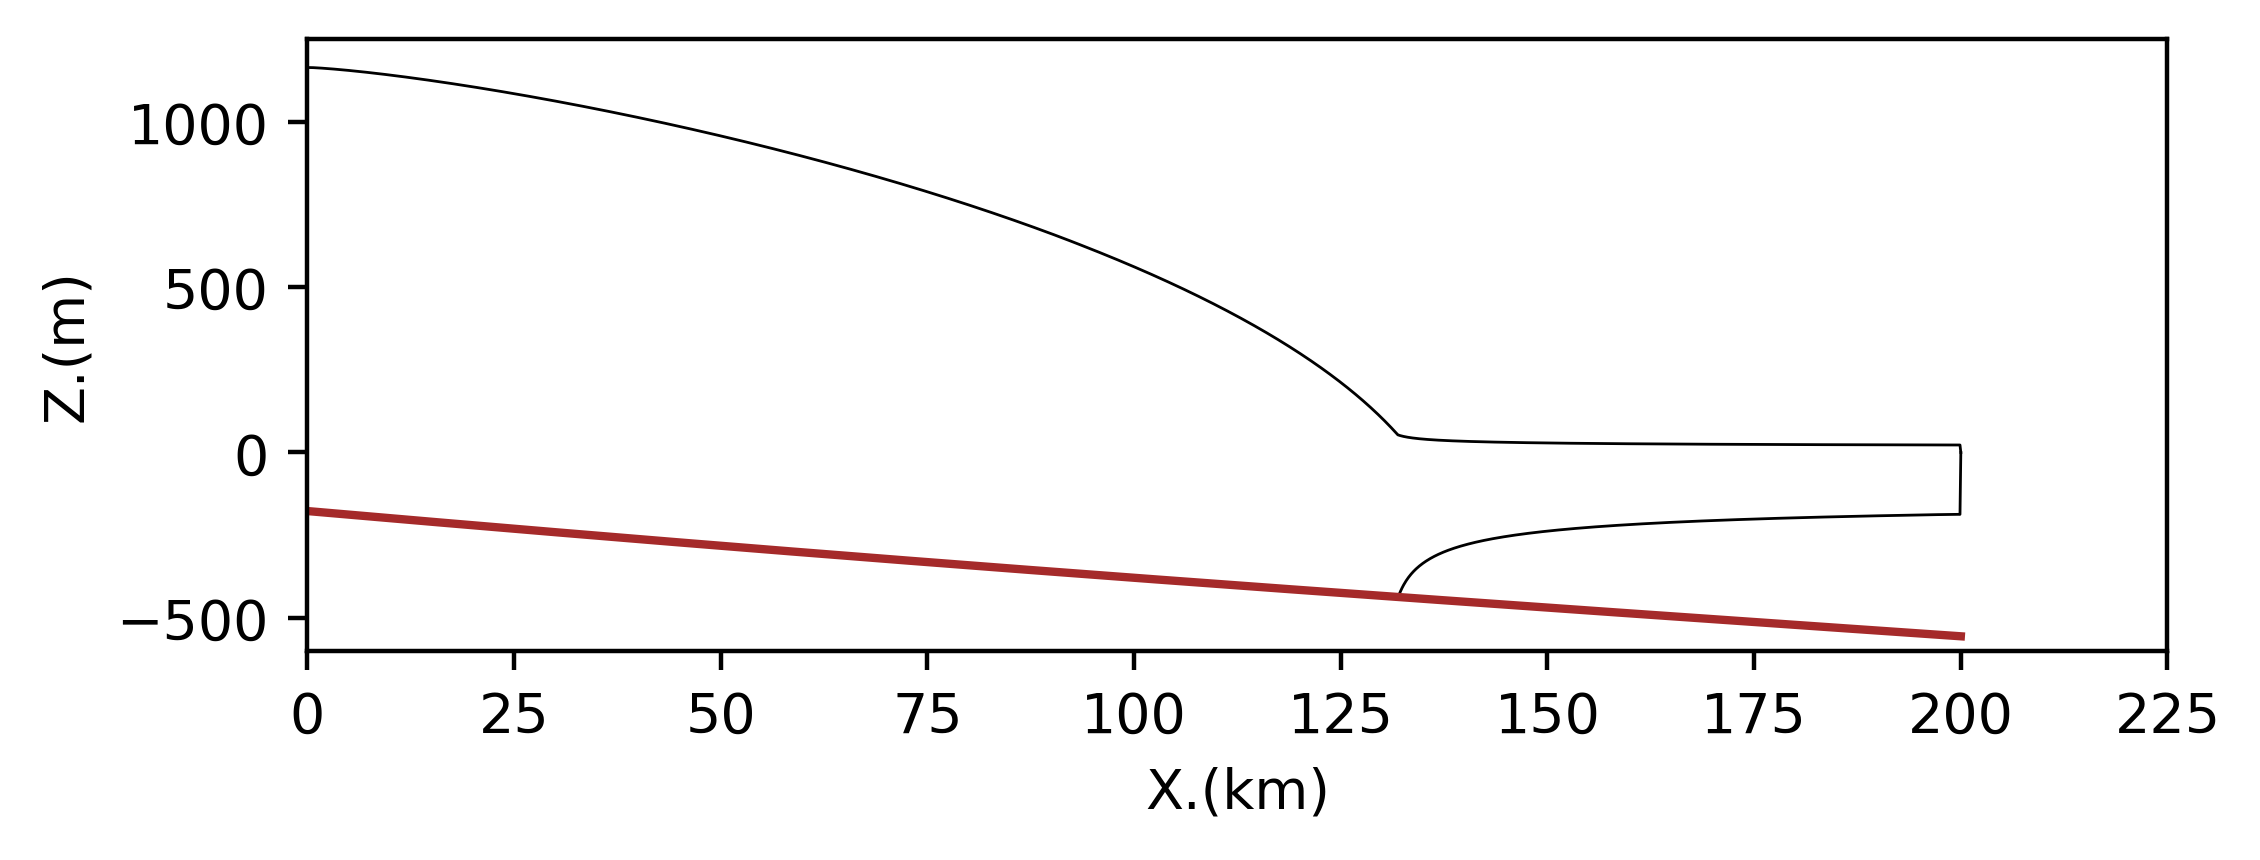
\includegraphics[width=8.3cm]{../figures/overview.png}
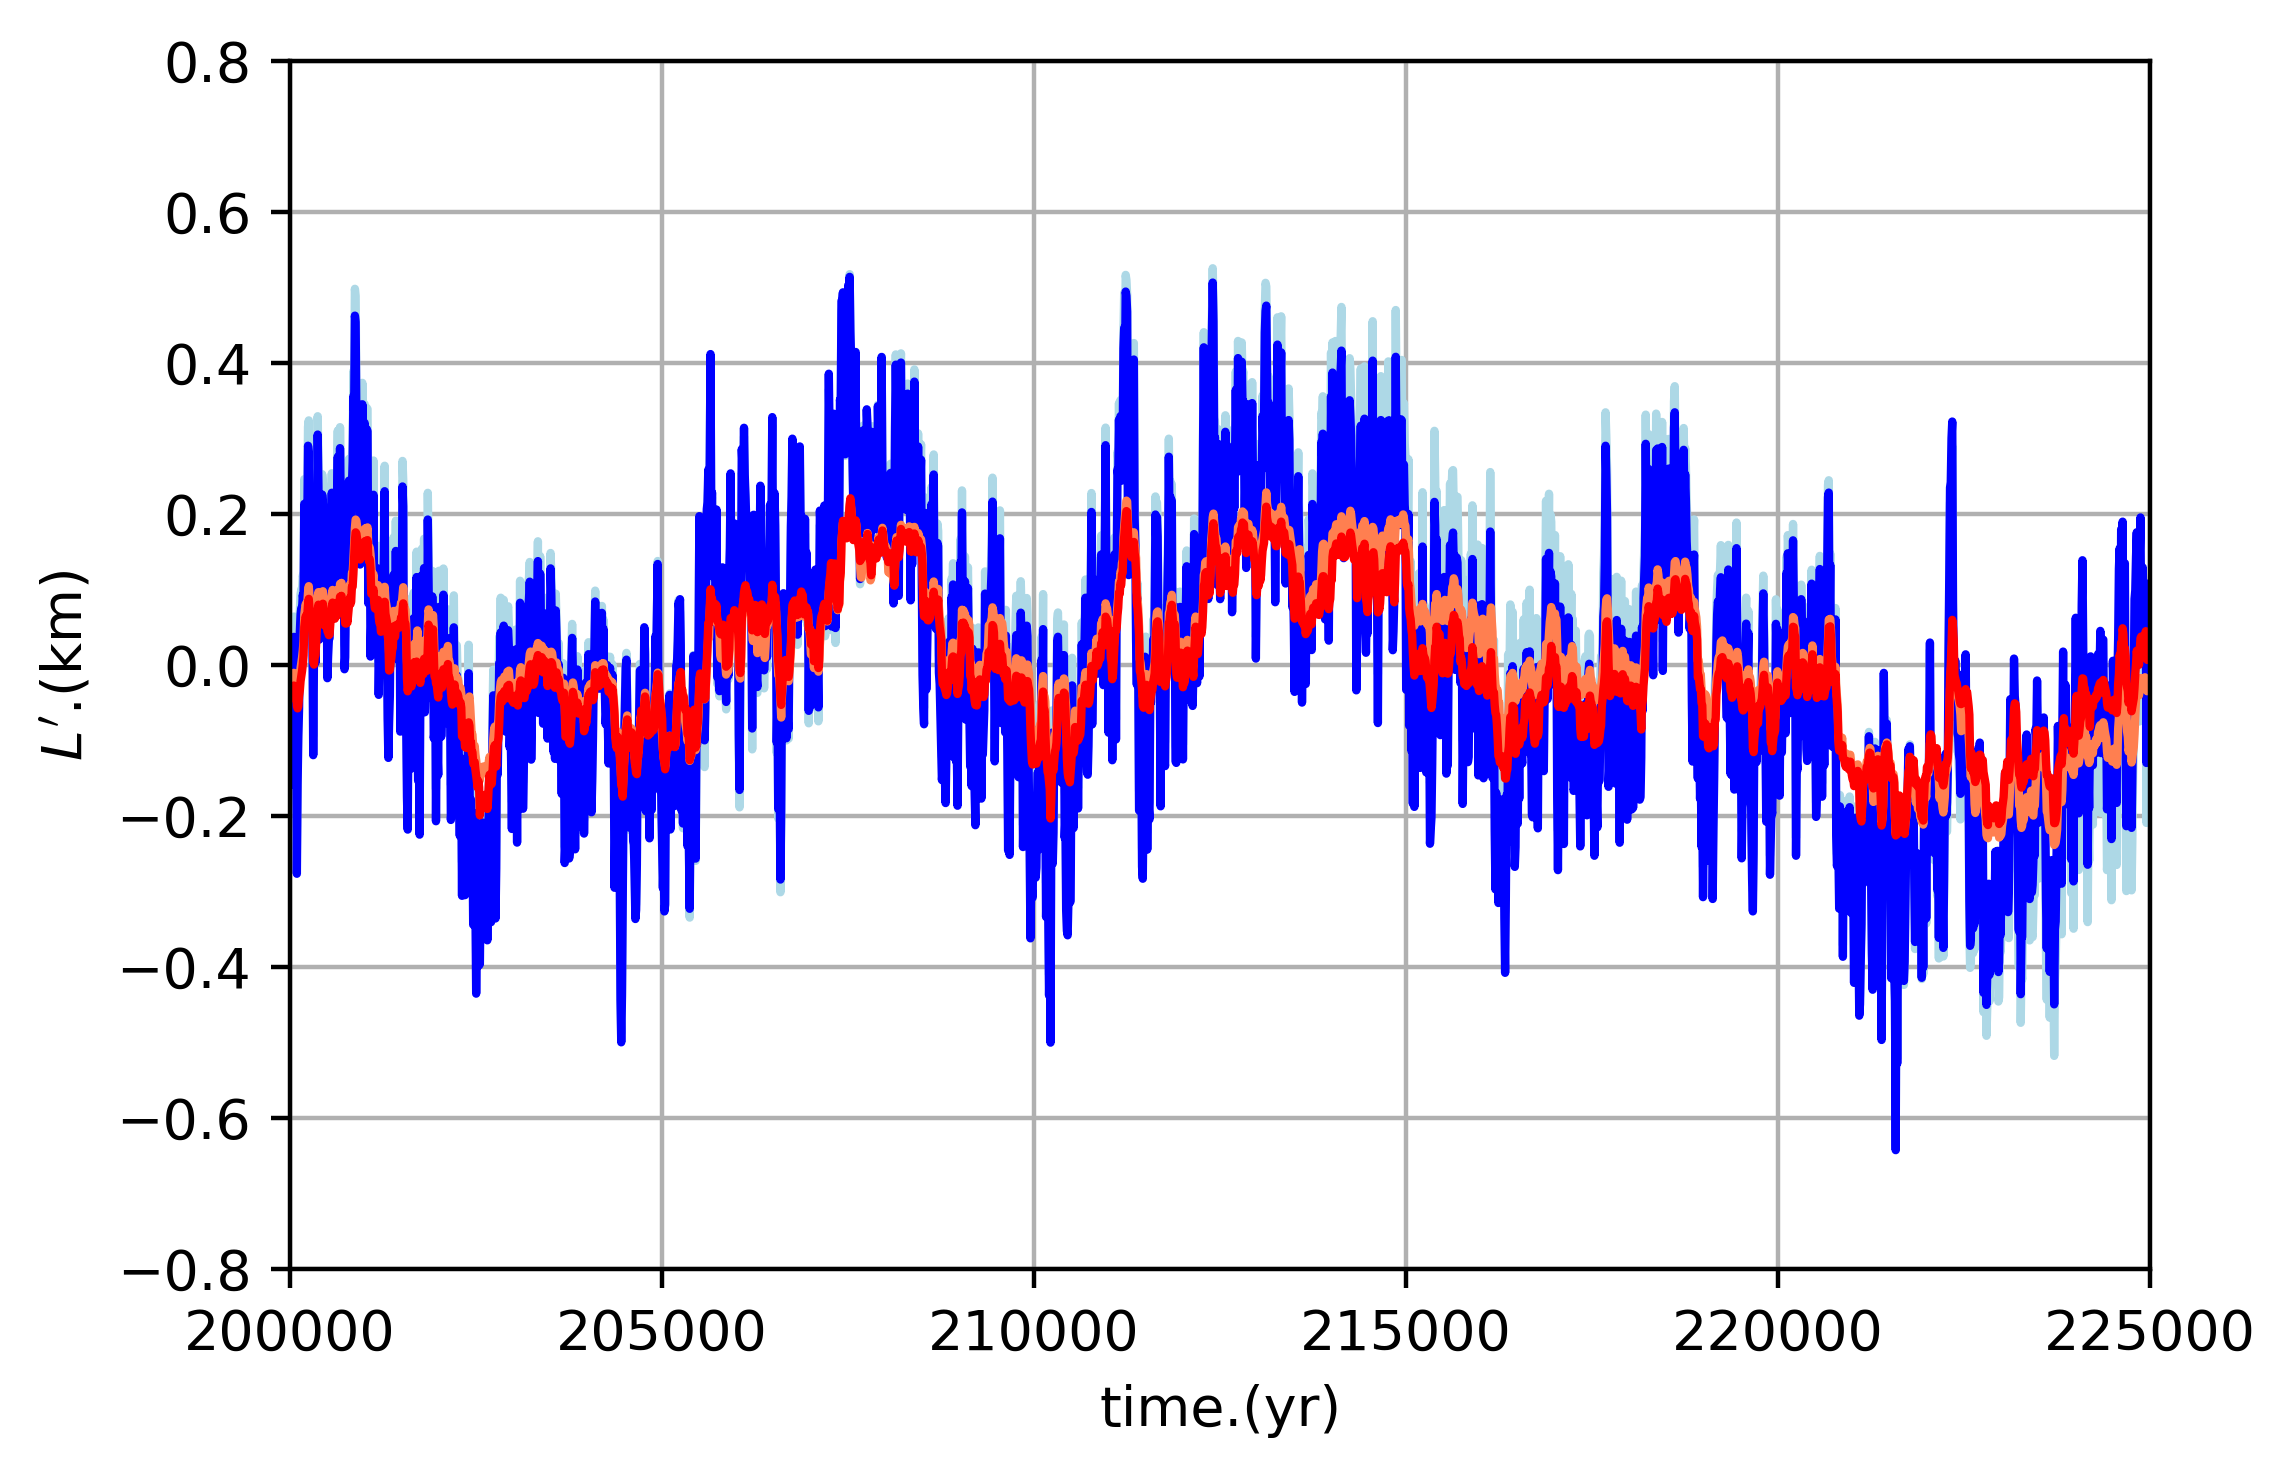
\includegraphics[width=8.3cm]{../figures/length_perturbation_timeseries.png}
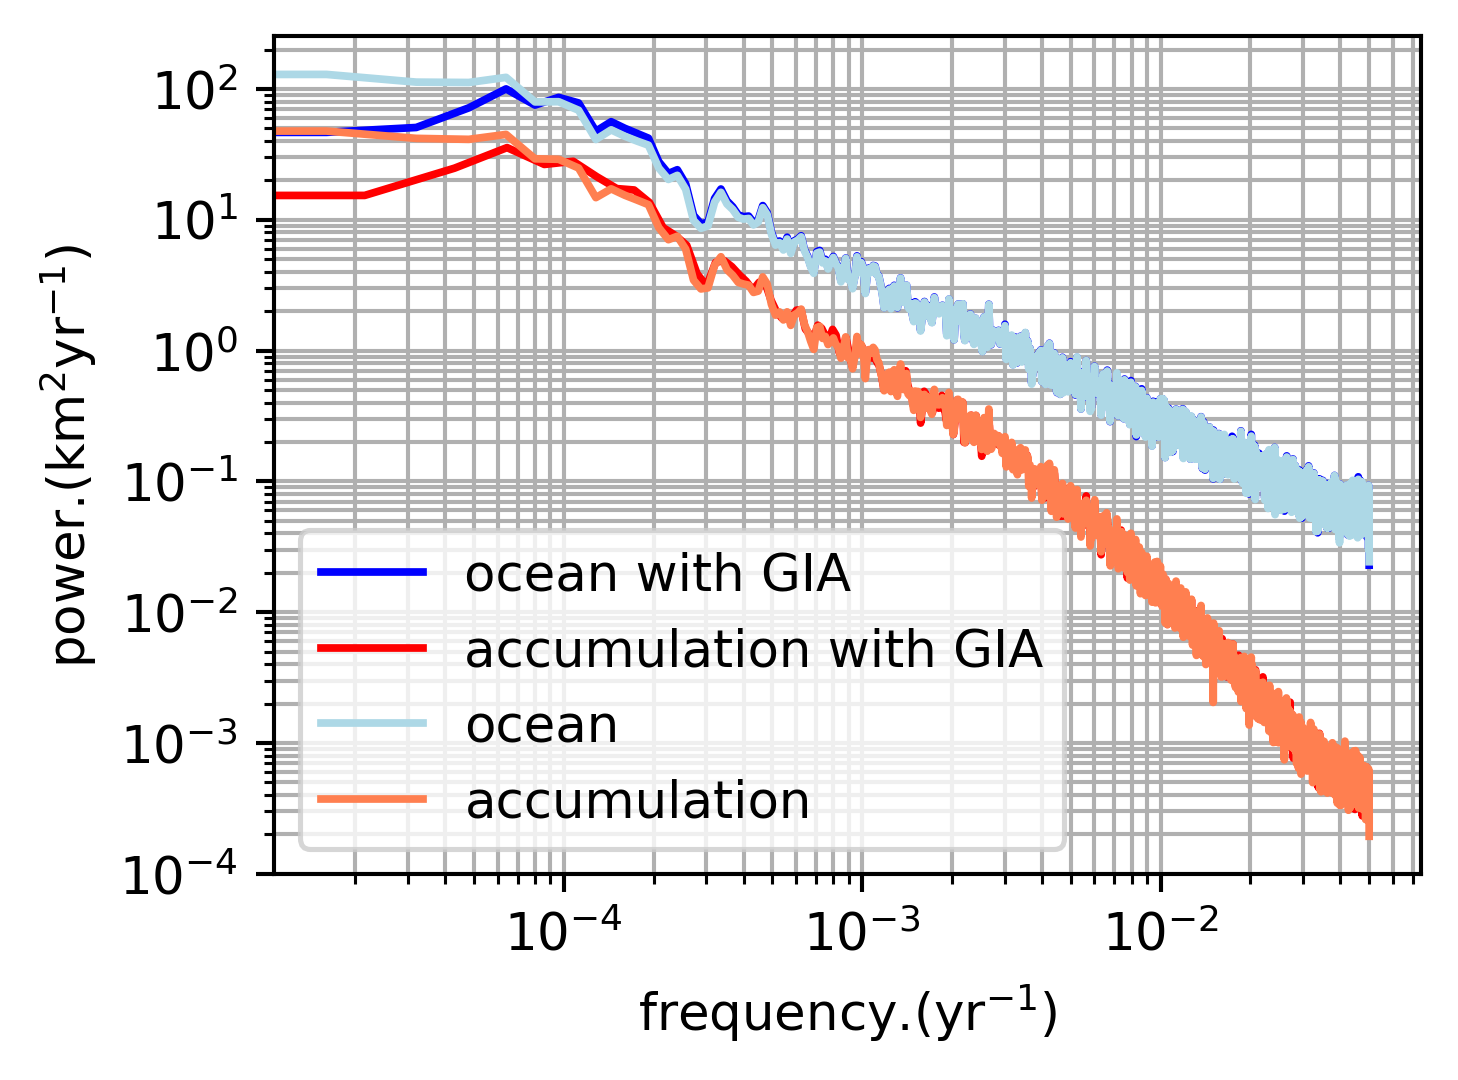
\includegraphics[width=8.3cm]{../figures/power_spectra.png}
\caption{ Glacier-solid earth model schematic and response to forcing. (a) the steady state profile of the ice-sheet bedrock system as simulated by the idealized flowline model. (b) Response of the flowline model to step changes in surface mass balance flux with and without the bedrock adjustment. (c) White noise time series of perturbation. (d) Length response to perturbations. (e) The power spectral density of glacier length perturbations.}
\end{figure}



We apply forcing variability as interannual white noise, which by definition has equal power at all frequencies and no interannual persistence. We apply the exact same white-noise time series as perturbations in the grounding line flux coefficient or the surface mass balance anomalies but with the opposite sign so that the corresponding ice-volume anomalies match. The anomaly time series are scaled to have standard deviations equal to $20\%$ of the mean values. Figure 2b shows the resulting length responses and Figure 2e shows the resulting power spectral density of length change.  
Because white-noise forcing has a flat power spectrum, the shapes of the response spectra reveal the glacier's filtering properties.
For both types of forcing, the glacier acts as a band-pass filter on the imposed climate anomalies, producing kilometer-scale fluctuations with clear persistence that are damped at low frequencies compared to the rigid bedrock system as the bed slope adjustment tends to guide the glacier back to equilibrium.

\subsection{Kinematic model}

To further understand the behavior of the ice-sheet bedrock system, we simplify our conceptual model to understand the coupling of state variables that represent the glacier length, interior thickness, and bedrock slope.
Ice-sheet mass change can be described in two stages for an idealized stable ice-sheet (Robel et al 2018; Christian et al 2020).
In the first stage, accumulation falls in the interior and flows under its own weight towards the outlet glacier margins.
The surface mass balance flux ($L\cdot S$) is modified by the interior flux, $Q$, according to the partitioning of stress accommodated by internal deformation and basal traction.
The interior reservoir of the ice-sheet drains according to this interior flux until it reaches the second stage where stresses change as the glacier goes afloat giving rise to a kinematic grounding line flux $Q_g$, that depends nonlinearly on the grounding zone ice thickness, $h_g$,
\begin{align}
Q_g=\Omega h_g^\beta.
\end{align}
 Two coupled equations capture the response of $H$, the interior thickness, and $L$, the glacier length, as they relax towards a steady state that balances all three fluxes:
 \begin{align}
 \frac{dL}{dt} &=\frac{1}{hg}(Q-Q_g) \\
\frac{dH}{dt} &=S - \frac{Q}{L}-\frac{H}{h_g L}(Q-Q_g).& 
\end{align}
Descriptions of the kinematic fluxes ($L\cdot S, Q, Q_g$) with time series of forcing (i.e. surface mass balance, $S$ and ocean melt rate, $\Omega$) form a closed system of ordinary differential equations that describe variations in glacier thickness and length. 
To represent the coupled response of the ice-sheet-lithosphere system, requires a third equation to capture the adjustment of the bedrock.
To approximate the change in bedrock slope due to changes in glacier geometry, we calculate the new equilibrium slope based on the ice-sheet-ocean thickness profile and current deflection of the lithosphere. 
The change in bedrock slope defines the new bed geometry and grounding line position, introducing a third stage to the outlet glacier model.
The new system of equations that define the glacier-bedrock system are:
\begin{align}
    \frac{dL}{dt} & = \frac{1}{h_g(L,b_x)}\cdot(Q(L,H)-Q_g(L,b_x)), \\
    \frac{dH}{dt} & = S-\frac{Q_g(L,b_x)}{L}-\frac{H}{h_g(L,b_x) L} \cdot (Q(L,H)-Q_g(L,b_x)), \\
    \frac{db_x}{dt} & = -\frac{1}{\tau}(b_x - b_{x_0}).
\end{align}

\begin{table}[h]
    \begin{tabular}{lll}
        Symbol & Meaning \\
        \hline
        $L$ & glacier length \\
        $H$ & interior thickness \\
        $b_x$ & bedrock slope \\
        $h_g$ & grounding zone thickness \\
        $Q$ & interior flux \\
        $Q_g$ & grounding zone flux \\
        $b_{x_0}$ & equilibrium bedrock slope \\
        $\tau$ & response time of solid earth  \\
        \\
        
    \end{tabular}
    
    \caption{Mathematical symbols and descriptions of parameters used in the kinematic ice-sheet bedrock model.}
\end{table}

The outlet glacier model equations (8-10)  can be linearized to understand changes in the glacier length, thickness, and bedrock slope about a local equilibrium position $\bar{L}, \bar{H}$, and $\bar{b_x}$. At this stable equilibrium, the interior and grounding zone fluxes balance one another and the evolution of fluctuations about the average length, thickness and slope can be written in vector form as:

\begin{align}
\frac{\partial}{\partial t}
 \begin{bmatrix} L' \\ H' \\ b_x' \end{bmatrix}
 &=
  \begin{bmatrix}
   A_L & A_H & A_{b_x}  \\
   B_L & B_H& B_{b_x} \\
   C_L & C_H & C_{b_x}
   \end{bmatrix}
    \begin{bmatrix} L' \\ H' \\ b_x' \end{bmatrix}
    +
    \begin{bmatrix} \sigma_H \\  \sigma_L \\ \sigma_{b_x} \end{bmatrix} f(t)&
\end{align}
\begin{align}
\bf{Y} = 
 \begin{bmatrix} L' \\ H' \\ b_x' \end{bmatrix};
 \bf{J}=
  \begin{bmatrix}
   A_L & A_H & A_{b_x}  \\
   B_L & B_H& B_{b_x} \\
   C_L & C_H & C_{b_x}
   \end{bmatrix};
  \bf{S}=
    \begin{bmatrix} \sigma_H \\  \sigma_L \\ \sigma_{b_x} \end{bmatrix}&
\end{align}




where $A_H, A_L, A_{b_x}, B_H, B_L, B_{b_x}, C_H, C_L,$ and $C_{b_x}$ describe the couplings between length, thickness, and bed-slope changes (see appendix for coefficient solutions), and $\sigma_H$, $\sigma_L$, and $\sigma_{b_x}$ describe the projection of terminus and interior climate forcing on each state variable. For interior surface mass balance forcing and grounding-line forcing, the projection can be written as

\begin{align}
\bf{S}_{precip} =   \begin{bmatrix} 1 \\ 0 \\ 0 \end{bmatrix}; \space
\bf{S}_{grounding} =   \begin{bmatrix} \bar{h_g}^{-1} \\ \bar{L}^{-1}\left(\frac{\bar{H}}{\bar{h_g}}-1\right) \\ 0 \end{bmatrix}.
\end{align}



The coupling described by each coefficient does not take a simple form because of the additional feedback with the bedrock slope, so we substitute representative glacier geometry, rheology and sliding parameter values into the vectorized system of equations to understand the solution character empirically. 


\section{Interpretations}


\begin{table}[h]
    \begin{tabular}{llll}
        \hline
        \bf{Parameter} & \bf{Glacier 1} & \bf{Glacier 2} & \bf{Glacier 3} \\
        \hline
        Surface mass balance, $\bar{S}$ & $0.5$ & $0.6$ & $0.3$ \\
        Buttressing, $\theta$ & $0.7$ &  $0.75$ & $0.6$ \\
        asthenosphere relaxation time scale, $\tau$ & $3000$ & $2000$ & $4000$ \\
        Bed elev. at divide, $b_0$ & $-100$ & $150$ & $100$  \\
        \hline
        \bf{Steady State} \\
        \hline
        equilibrium length, $\bar{L}$ ($km$) &  $182$  & $212$ & $700$ \\
        equilibrium thickness, $\bar{H}$ ($m$) & $1412$ & $1569$ & $2814$ \\
         equilibrium bed slope, $\bar{b_x}$ & $-2 \times 10^{-3}$ & $-3 \times 10^{-3}$ & $-1 \times 10^{-3}$ \\
        grounding line thickness, $\bar{h_g}$ ($m$) & $526$ & $545$ & $673$ \\
        fast response time, $\tau_f$ (yr) & $75$ & 60 & 150 \\
        slow response time, $\tau_s$ (yr) & $765$ & 1020 & 1505 \\
        periodic response time, $\tau_p$ (yr) & $1670$ & 2152 & 3157 \\
        \hline
        \\
        
    \end{tabular}
    
    \caption{Parameters varied between three idealized glacier geometries, along with the solution for the linearized model.}
\end{table}

With the addition of the third-stage wherein the bedrock slope is allowed to respond with length and thickness change, the linearized glacier-bedrock model's eigenmodes are complex exponentially decaying functions composed of three characteristic timescales $\tau_f$, $\tau_s$ and $\tau_p$. The complex solutions introduce a third timescale that describes the frequency of damped oscillation (periodic motion described by $\tau_p$), and agrees with the damped resonance we observe from dynamic flow-line model simulations. We project the vector-form equation for the system onto the system eigenmodes, which can be written as simple one-dimensional linear ordinary differential equations for which we can write the green's function in the time domain, the power spectral density, and the covariance function explicitly and project onto the state variables to further understand the character of the response (see appendix for details). There are two factors that govern the state variable response for the system eigenmodes. The relative projection of each eigenmode onto one of the state variables, and the relative projection of external forcing onto each eigenmode.


\begin{figure}[t]
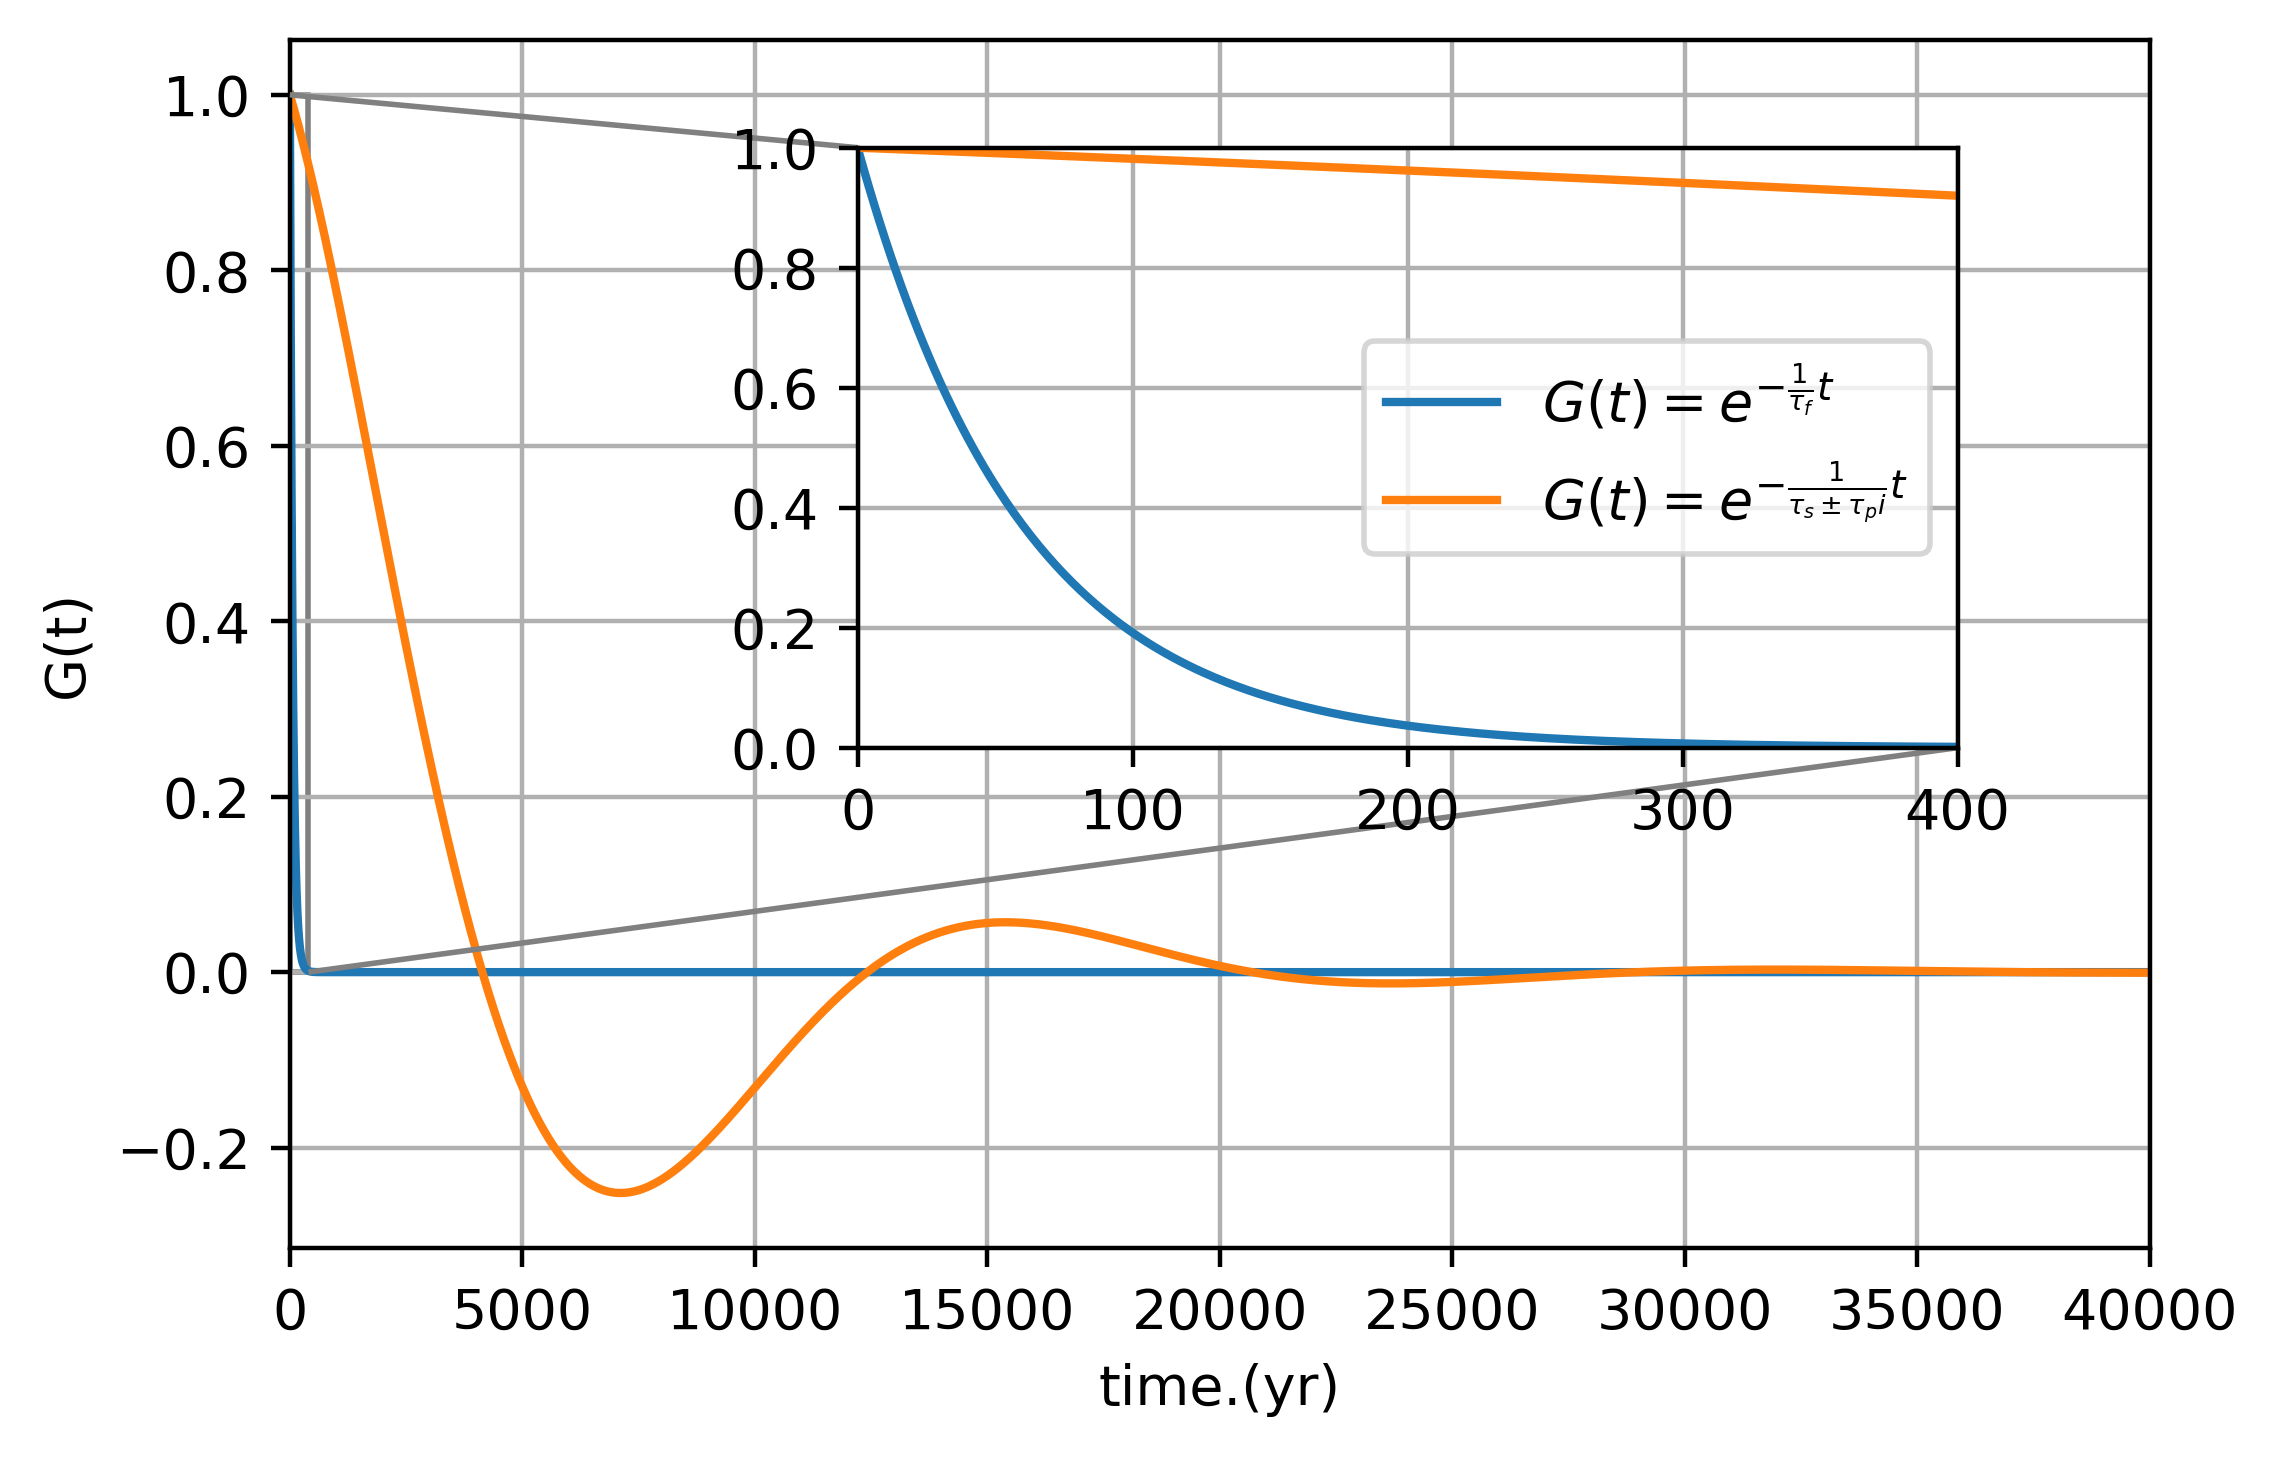
\includegraphics[width=8.3cm]{../figures/greens_function.png}
\caption{Model response from theoretical eigenmode decomposition. (a) Green's function for the system eigenmodes (b)
The left column is the length response to precipitation forcing ($\Delta S = −0.2$). 
The right column is the length response to Grounding Line forcing ($\Delta Q_g = 0.2$).
The projections of the eigenmodes onto the $H, L$, and $b_x$ are identical. The only difference comes from ($\sigma_H, \sigma_L, \sigma_{b_x}$) which affects how much each type of forcing excites each eigenmode.}
\end{figure}



Figures ** demonstrate that the inclusion of isostatic adjustment significantly changes the behavior of marine-terminating outlet glaciers. 
In the next section, we examine the consequences of filtering properties of the coupled ice-sheet-bedrock system for two key questions in glaciology: 
How does damping at non-resonant frequencies affect the spectra of ice volume variability preserved in proxy records?
And how could the resonant response of the glacier to forcing variability, in turn, affect the climate system?


\subsection{Damping and Resonance}

This section is underdeveloped in my head. I think we could aim to characterize the effect of damping and how the glaciological filter manifests in time series of glacier volume change (of interest to paleo climate communities)? The perspective could adopt a detectability approach (how sensitive do proxy records need to be to see the affect of isostacy?), or instead focus on hypothetical/realistic time series and look to see how the filter affects length change/inferences of past climate.

\subsection{Climate-bedrock Feedbacks}

Few signals in the geologic record have captured the attention of the paleoclimate, and glaciology communities more than "Heinrich events" documented as anomalous occurrences of ice-rafted debris deposited in the North Atlantic during the last glacial.
While the mechanism that drives these events remains a matter of debate, aspects of their character preserved in the proxy record are clear:
The climate-ice sheet coupling appears to be phase locked with striking coincidence with the pattern of climate fluctuations documented from ice cores, and there is good evidence for global climate changes coincident with each event.


\section{Summary and Discussion}

We've made a number of simplifying assumptions throughout our study. 
We do not include elastic contributions to the glacier bedrock system in our linearized model.
There are also other processes that affect bedrock geometry that we do not account for in either model.
These include thermal subsidence following tectonic extension (likely a key process in West Antarctica), and glacially driven erosion and sedimentation and accompanying isostatic response.
These processes take place on timescales that are substantially lower frequencies than the e-folding times and oscillation periods we explore in this study.
We also exclude feedbacks between ice sheet-bedrock geometry and forcing, which can change the melt rate, and surface mass balance as the glacier and bedrock geometry change.


\conclusions  
Our simple modeling demonstrates a subtle feedback between multi-milenia climate variability and the modulation of marine ice-sheet bedrock that tends to stabilize the marine ice-sheet system by damping low frequency oscillations in glacier thickness and glacier length relative to simulations that assume no bedrock response. 
The same feedback also amplifies oscillations in glacier length at the resonant frequency of the bedrock.


%% The following commands are for the statements about the availability of data sets and/or software code corresponding to the manuscript.
%% It is strongly recommended to make use of these sections in case data sets and/or software code have been part of your research the article is based on.

\codedataavailability{The code used to run the simulations included in the text is freely available at https://github.com/hoffmaao/gia2stage (last accessed April 20 2021).} 


%\dataavailability{TEXT} %% use this section when having only data sets available


%\videosupplement{TEXT} %% use this section when having video supplements available


\appendix
\section{Derivation of linear model}    %% Appendix A

The coefficients of the system operator matrix
\begin{multline*}
    A_L = \frac{-\bar{H}^\alpha \bar{L}^{-1 - \gamma} \gamma \nu - \bar{m} \beta \lambda \Omega((b_0 + \bar{L} \bar{m}) \lambda)^{-1 + \beta}}{(b_0 +\bar{L} \bar{m}) \lambda} + \frac{(\bar{m} (\bar{H}^\alpha \bar{L}^-\gamma \nu + \Omega(b_0 + \bar{L} \bar{m}) \lambda)^\beta}{(b_0+ \bar{L} \bar{m})^2 \lambda}, \\
    A_H =  \frac{- \bar{H}^{-1 + \alpha} \bar{L}^-\gamma \alpha \nu}{(b_0 + \bar{L} \bar{m}) \lambda}, \\
    A_m =  \frac{-((\bar{L} \beta (-(b_0 + \bar{L} \bar{m}) \lambda)^{-1 + \beta} \Omega)}{b_0 + \bar{L} \bar{m}} + \frac{(\bar{L} (\bar{H}^\alpha \bar{L}^-\gamma \nu - (-(b_0 + \bar{L} \bar{m}) \lambda)^\beta \Omega))}{(b_0 + \bar{L} \bar{m})^2 \lambda}, \\
    B_L = \frac{\bar{m} \beta \lambda (-(b_0 + \bar{L} \bar{m}) \lambda)^{-1 + \beta} \Omega)}{\bar{L}} + \frac{((-(b_0 + \bar{L} \bar{m}) \lambda)^\beta \Omega)}{\bar{L}^2} + \frac{(\bar{H} (-\bar{H}^\alpha \bar{L}^(-1 - \gamma) \gamma \nu + \bar{m} \beta \lambda (-(b_0 + \bar{L} \bar{m}) \lambda)^(-1 + \beta) \Omega))}{\bar{L} (b_0 + \bar{L} \bar{m}) \lambda} \\
    - \frac{(\bar{H} \bar{m} (\bar{H}^\alpha \bar{L}^-\gamma \nu - (-(b_0 + \bar{L} \bar{m}) \lambda)^\beta \Omega))}{\bar{L} (b_0 + \bar{L} \bar{m})^2 \lambda} - \frac{(\bar{H} (\bar{H}^\alpha \bar{L}^-\gamma \nu - (-(b_0 + \bar{L} \bar{m}) \lambda)^\beta] \Omega))}{\bar{L}^2 (b_0 + \bar{L} \bar{m}) \lambda}, \\
    B_H = \frac{\bar{H}^\alpha \bar{L}^(-1 - \gamma) \alpha \nu}{(b_0 + \bar{L} \bar{m}) \lambda} + \frac{\bar{H}^\alpha \bar{L}^-\gamma \nu - (-(b_0 + \bar{L} \bar{m}) \lambda)^\beta \Omega}{\bar{L} (b_0 +\bar{ L} \bar{m}) \lambda}, \\
    B_m = \frac{\bar{H} \beta (-(b_0 + \bar{L} \bar{m}) \lambda)^{-1 + \beta} \Omega}{b_0 + \bar{L} \bar{m}} + \beta \lambda (-(b_0 + \bar{L} \bar{m}) \lambda)^{-1 + \beta} \Omega - \frac{\bar{H} (\bar{H}^\alpha \bar{L}^-\gamma \nu - (-(b_0 + \bar{L} \bar{m}) \lambda)^\beta \Omega)}{(b_0 + \bar{L} \bar{m})^2 \lambda}, \\
    C_L =-\frac{-\frac{1}{3} \bar{L} \bar{m} \kappa - 
  \frac{1}{3} (-b_0 + 2\bar{H} + \bar{L} \bar{m}) \kappa}{\tau}, \\
    C_H=\frac{2 \bar{L} \kappa}{3 \tau}, \\
    C_m=-\frac{1 - \frac{(\bar{L}^2 \kappa)}{3}}{\tau}. \\
\end{multline*}
     
\section{Eigenmode decomposition}     %% Appendix A1, A2, etc.
We can diagonalize the system's operator matrix 
\begin{align}
\bf{J} &= \bf{P} \Lambda \bf{P^{-1}},& \\
\Lambda &=  \begin{bmatrix}
   -\alpha_1 & 0 & 0  \\
   0 & -\alpha_2 & 0 \\
   0 & 0 & -\alpha_3
   \end{bmatrix}&
\end{align}
where $\bf{P}$, $\bf{P^{-1}}$ are the projection matrices, so called because they project between the actual state space of the system ($H, L, b_x$), and $\bf{\Lambda}$ is the diagonal matrix containing the system eigenvalues.

\begin{align}
\frac{d}{dt} m_1 = -\alpha_1 m_1 + \sigma_1 f(t)\\
\frac{d}{dt} m_2 = -\alpha_2 m_2 + \sigma_2 f(t)\\
\frac{d}{dt} m_3 = -\alpha_3 m_3 + \sigma_3 f(t)
\end{align}



\noappendix       %% use this to mark the end of the appendix section. Otherwise the figures might be numbered incorrectly (e.g. 10 instead of 1).

%% Regarding figures and tables in appendices, the following two options are possible depending on your general handling of figures and tables in the manuscript environment:

%% Option 1: If you sorted all figures and tables into the sections of the text, please also sort the appendix figures and appendix tables into the respective appendix sections.
%% They will be correctly named automatically.

%% Option 2: If you put all figures after the reference list, please insert appendix tables and figures after the normal tables and figures.
%% To rename them correctly to A1, A2, etc., please add the following commands in front of them:

\appendixfigures  %% needs to be added in front of appendix figures

\appendixtables   %% needs to be added in front of appendix tables

%% Please add \clearpage between each table and/or figure. Further guidelines on figures and tables can be found below.



\authorcontribution{AOH wrote the paper and all authors contributed revisions.} %% this section is mandatory

\begin{acknowledgements}
AOH was supported by NASA FINESST grant progran ()
\end{acknowledgements}




%% REFERENCES

%% The reference list is compiled as follows:

\begin{thebibliography}{}

\bibitem[AUTHOR(YEAR)]{LABEL1}
REFERENCE 1

\bibitem[AUTHOR(YEAR)]{LABEL2}
REFERENCE 2

\end{thebibliography}

%% Since the Copernicus LaTeX package includes the BibTeX style file copernicus.bst,
%% authors experienced with BibTeX only have to include the following two lines:
%%
%% \bibliographystyle{copernicus}
%% \bibliography{example.bib}
%%
%% URLs and DOIs can be entered in your BibTeX file as:
%%
%% URL = {http://www.xyz.org/~jones/idx_g.htm}
%% DOI = {10.5194/xyz}


%% LITERATURE CITATIONS
%%
%% command                        & example result
%% \citet{jones90}|               & Jones et al. (1990)
%% \citep{jones90}|               & (Jones et al., 1990)
%% \citep{jones90,jones93}|       & (Jones et al., 1990, 1993)
%% \citep[p.~32]{jones90}|        & (Jones et al., 1990, p.~32)
%% \citep[e.g.,][]{jones90}|      & (e.g., Jones et al., 1990)
%% \citep[e.g.,][p.~32]{jones90}| & (e.g., Jones et al., 1990, p.~32)
%% \citeauthor{jones90}|          & Jones et al.
%% \citeyear{jones90}|            & 1990



%% FIGURES

%% When figures and tables are placed at the end of the MS (article in one-column style), please add \clearpage
%% between bibliography and first table and/or figure as well as between each table and/or figure.

% The figure files should be labelled correctly with Arabic numerals (e.g. fig01.jpg, fig02.png).


%% ONE-COLUMN FIGURES

%%f
%\begin{figure}[t]
%\includegraphics[width=8.3cm]{FILE NAME}
%\caption{TEXT}
%\end{figure}
%
%%% TWO-COLUMN FIGURES
%
%%f
%\begin{figure*}[t]
%\includegraphics[width=12cm]{FILE NAME}
%\caption{TEXT}
%\end{figure*}
%
%
%%% TABLES
%%%
%%% The different columns must be seperated with a & command and should
%%% end with \\ to identify the column brake.
%
%%% ONE-COLUMN TABLE
%
%%t
%\begin{table}[t]
%\caption{TEXT}
%\begin{tabular}{column = lcr}
%\tophline
%
%\middlehline
%
%\bottomhline
%\end{tabular}
%\belowtable{} % Table Footnotes
%\end{table}
%
%%% TWO-COLUMN TABLE
%
%%t
%\begin{table*}[t]
%\caption{TEXT}
%\begin{tabular}{column = lcr}
%\tophline
%
%\middlehline
%
%\bottomhline
%\end{tabular}
%\belowtable{} % Table Footnotes
%\end{table*}
%
%%% LANDSCAPE TABLE
%
%%t
%\begin{sidewaystable*}[t]
%\caption{TEXT}
%\begin{tabular}{column = lcr}
%\tophline
%
%\middlehline
%
%\bottomhline
%\end{tabular}
%\belowtable{} % Table Footnotes
%\end{sidewaystable*}
%
%
%%% MATHEMATICAL EXPRESSIONS
%
%%% All papers typeset by Copernicus Publications follow the math typesetting regulations
%%% given by the IUPAC Green Book (IUPAC: Quantities, Units and Symbols in Physical Chemistry,
%%% 2nd Edn., Blackwell Science, available at: http://old.iupac.org/publications/books/gbook/green_book_2ed.pdf, 1993).
%%%
%%% Physical quantities/variables are typeset in italic font (t for time, T for Temperature)
%%% Indices which are not defined are typeset in italic font (x, y, z, a, b, c)
%%% Items/objects which are defined are typeset in roman font (Car A, Car B)
%%% Descriptions/specifications which are defined by itself are typeset in roman font (abs, rel, ref, tot, net, ice)
%%% Abbreviations from 2 letters are typeset in roman font (RH, LAI)
%%% Vectors are identified in bold italic font using \vec{x}
%%% Matrices are identified in bold roman font
%%% Multiplication signs are typeset using the LaTeX commands \times (for vector products, grids, and exponential notations) or \cdot
%%% The character * should not be applied as mutliplication sign
%
%
%%% EQUATIONS
%
%%% Single-row equation
%
%\begin{equation}
%
%\end{equation}
%
%%% Multiline equation
%
%\begin{align}
%& 3 + 5 = 8\\
%& 3 + 5 = 8\\
%& 3 + 5 = 8
%\end{align}
%
%
%%% MATRICES
%
%\begin{matrix}
%x & y & z\\
%x & y & z\\
%x & y & z\\
%\end{matrix}
%
%
%%% ALGORITHM
%
%\begin{algorithm}
%\caption{...}
%\label{a1}
%\begin{algorithmic}
%...
%\end{algorithmic}
%\end{algorithm}
%
%
%%% CHEMICAL FORMULAS AND REACTIONS
%
%%% For formulas embedded in the text, please use \chem{}
%
%%% The reaction environment creates labels including the letter R, i.e. (R1), (R2), etc.
%
%\begin{reaction}
%%% \rightarrow should be used for normal (one-way) chemical reactions
%%% \rightleftharpoons should be used for equilibria
%%% \leftrightarrow should be used for resonance structures
%\end{reaction}
%
%
%%% PHYSICAL UNITS
%%%
%%% Please use \unit{} and apply the exponential notation


\end{document}
